\begin{figure}[htbp]
    \centering
    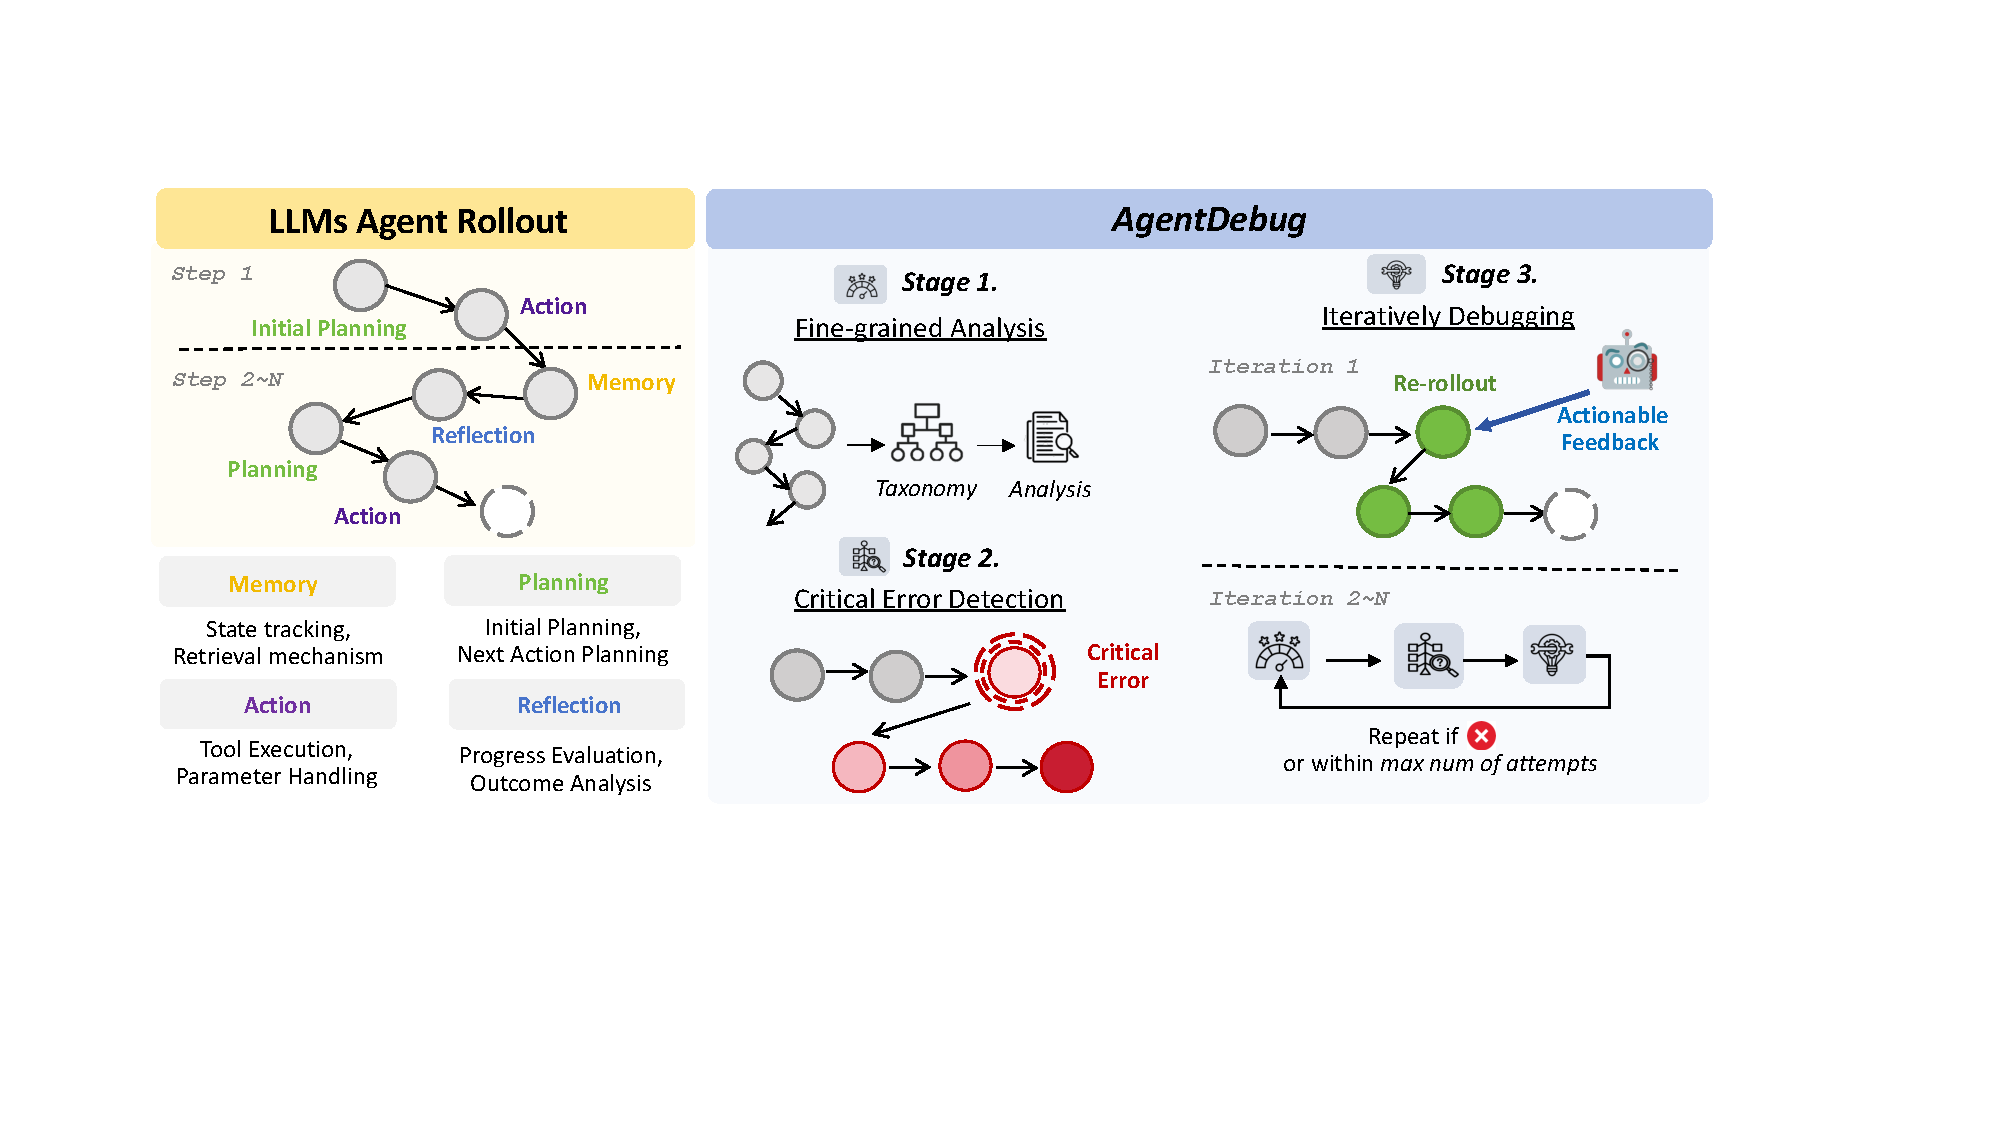
\includegraphics[width=1\linewidth]{figures/method.pdf}
    \caption{\textbf{Overview of proposed \ModelName{}.} (Left) Normal rollouts cycle through memory, planning, reflection, and action. (Right) \ModelName{} debugs trajectories in three stages: (1) comprehensive scoring, (2) critical error detection, and (3) iterative re-rollouts with actionable feedback to flip failures into successes. }
    \label{fig:method}
\end{figure}

\begin{algorithm}[h]
\caption{\ModelName{} Framework with Agent Workflow}
\label{alg:model}
\begin{algorithmic}[1]
\Require Trajectory $\tau$, scoring functions $\{g_m\}$, budget $B$
\State Compute $\sigma_t^m=g_m(s_t,a_t)$, map to \AET{} error types $e_t^m$
\State Aggregate $\Sigma(\tau)=\tfrac{1}{T}\sum_t \sum_m w_m\sigma_t^m$
\If{$y(\tau)=1$} \Return $\tau$ \EndIf
\State $t^\ast \gets \arg\min_t \{ y(\tau^{(t \to \hat{a}_t)})=1 \}$
\State $\phi_{t^\ast}\gets\psi(s_{t^\ast},a_{t^\ast},e_{t^\ast})$
\For{$k=1$ to $B$}
    \State $\tau^{(k+1)}\gets\text{ReRollout}(\tau^{(k)},\phi_{t^\ast}^{(k)})$
    \If{$y(\tau^{(k+1)})=1$} \Return $\tau^{(k+1)}$ \EndIf
\EndFor
\State \Return Failure
\end{algorithmic}
\end{algorithm}



Given error analysis of agent failures, ideally we can develop an LLM with agentic workflow to refine LLM from failures.

We consider a generic agent formulation for the rollout agent which is prone to errors; then, we propose AgentDebug, a generic LLM that can fix the errors from the orignal rollout agent across different environments and rollout agent.
2

In low-resource academic setting, collecting a sufficient amount of data to potentially train an debug LLM will be cost prohibitive (est. cost XXX, with human labeling efforts). 
Instead, we developed an effective LLM workflow via prompt design that is cost efficient.
Note that our main purpose here is not to develop a SOTA debug LLM, instead, we aim to show that even with low-resource setting, our proposed TAXONOMY is highly effective in building a prompt based debug LLM workflow.

% \subsection{Trajectory Formulation}
\subsection{Key Modules of an LLM Agent}
We consider an agent $\pi$ interacting with an environment $\mathcal{E}$. A trajectory of length $T$ is:
\begin{equation}
    \tau = \{(s_1, a_1), (s_2, a_2), \dots, (s_T, a_T)\}, \quad s_t \in \mathcal{S},\; a_t \in \mathcal{A},
\end{equation}
where $\mathcal{S}$ and $\mathcal{A}$ denote the state and action spaces.  
Each action $a_t$ is generated through four modules:
\begin{equation}
    a_t = f_{\text{act}}\!\left(f_{\text{plan}}\!\left(f_{\text{refl}}\!\left(f_{\text{mem}}(s_t)\right)\right)\right),
\end{equation}
where $f_{\text{mem}}, f_{\text{plan}}, f_{\text{refl}}, f_{\text{act}}$ are the \textbf{Memory}, \textbf{Planning}, \textbf{Reflection}, and \textbf{Action} modules. We expect the agent may make errors in any the modules.

\subsection{\ModelName{} Framework}
\label{sec:modelname}

We design \ModelName{} as a debugging framework for single LLMs agent systems. As illustrated in Fig.~\ref{fig:method}, \ModelName{} explicitly analyzes full trajectories to:  
(i) assign comprehensive scores to every step and module,  
(ii) detect the earliest critical error, and  
(iii) guide re-rollouts with actionable feedback.  
The central principle is that correcting a single early decision can often flip the entire trajectory from failure to success.

As illustrated in Algorithm \ref{alg:model}, the inference procedure of \ModelName{} contains following stages:

\paragraph{Stage 1: Scoring with \AET{}.}  
We represent a trajectory $\tau=\{(s_1,a_1),\dots,(s_T,a_T)\}$ where each action is generated by  
\begin{equation}
    a_t = f_{\text{act}}(f_{\text{plan}}(f_{\text{refl}}(f_{\text{mem}}(s_t)))).
\end{equation}
Each module $m \in \{\text{mem},\text{plan},\text{refl},\text{act}\}$ is evaluated using  
\begin{equation}
    \sigma_t^m = g_m(s_t,a_t)\in[0,1],
\end{equation}
and combined into per-step and trajectory scores:  
\begin{equation}
    \sigma_t = \sum_m w_m\sigma_t^m, 
    \quad \Sigma(\tau)=\tfrac{1}{T}\sum_{t=1}^T\sigma_t.
\end{equation}
Importantly, each $\sigma_t^m$ is grounded in the \AET{} taxonomy, which maps steps to error types $e_t^m \in \mathcal{E}_{\text{err}}$ (e.g., planning constraint ignorance, action format error). This ensures that scoring is not only numeric but also interpretable in terms of root-cause categories.  

\paragraph{Stage 2: Critical Error Detection.}  
Let $y(\tau)\in\{0,1\}$ denote task outcome. We define the earliest critical step as  
\begin{equation}
    t^\ast = \arg\min_{t} \{\, y(\tau^{(t \to \hat{a}_t)})=1 \,\},
\end{equation}
where $\tau^{(t \to \hat{a}_t)}$ denotes a trajectory with corrected action $\hat{a}_t$. By linking $\hat{a}_t$ to the \AET{} error label $e_t^m$, \ModelName{} isolates not just \emph{when} the trajectory first goes wrong, but also \emph{why} (e.g., misrecall in memory, infeasible plan, or malformed action).  

\paragraph{Stage 3: Iterative Debugging.}  
For the detected error $e_{t^\ast}$, \ModelName{} generates targeted feedback
\begin{equation}
    \phi_{t^\ast} = \psi(s_{t^\ast},a_{t^\ast},e_{t^\ast}),
\end{equation}
and performs a re-rollout:
\begin{equation}
    \tau^{(k+1)} = \text{ReRollout}(\tau^{(k)},\phi_{t^\ast}^{(k)}), \quad k=1,\dots,B.
\end{equation}
The process repeats until $y(\tau^{(k+1)})=1$ or budget $B$ is reached. Theok feedback is conditioned on \AET{} categories, re-rollouts are interpretable and targeted rather than ad hoc.  


